\documentclass[aspectratio=169,12pt,t]{beamer}

% --- Theme: Metropolis (modern, clean) ---
\usetheme[progressbar=frametitle,numbering=fraction,block=fill]{metropolis}

% --- Fira Sans font (install texlive-fonts-extra if missing) ---
\IfFileExists{FiraSans.sty}{\usepackage[sfdefault]{FiraSans}}{}

% --- Light background with warm accent ---
\definecolor{mDarkTeal}{RGB}{35,55,59}
\definecolor{mLightBrown}{RGB}{235,228,216}
\definecolor{mAccent}{RGB}{140,70,20}

\setbeamercolor{normal text}{fg=mDarkTeal,bg=white}
\setbeamercolor{alerted text}{fg=mAccent}
\setbeamercolor{frametitle}{bg=mDarkTeal,fg=white}
\setbeamercolor{progress bar}{fg=mAccent,bg=mLightBrown}
\setbeamercolor{title separator}{fg=mAccent}
\setbeamercolor{progress bar in head/foot}{fg=mAccent,bg=mLightBrown}
\setbeamercolor{progress bar in section page}{fg=mAccent,bg=mLightBrown}

% --- Packages ---
\usepackage[utf8]{inputenc}
\usepackage{amsmath,amssymb,amsthm}
\usepackage{mathrsfs}
\usepackage{tikz}
\usetikzlibrary{arrows.meta,positioning,calc,decorations.pathreplacing,shapes,patterns,shadows.blur}
\usepackage{pgfplots}
\pgfplotsset{compat=1.18}

% --- Semi-transparent white highlight for text on top of background images ---
\usepackage[most]{tcolorbox}

% Inline highlight: \hl{short text}
\newtcbox{\hl}{%
  nobeforeafter, tcbox raise base,
  colback=white, opacityback=0.6,
  colframe=white, opacityframe=0,
  sharp corners, boxsep=2pt, left=3pt, right=3pt, top=2pt, bottom=2pt%
}

% Block highlight: \begin{hlbox} ... \end{hlbox}  (multi-line, paragraphs, itemize)
% Optional argument accepts any tcolorbox key, e.g. [width=0.6\linewidth]
\newtcolorbox{hlbox}[1][]{%
  enhanced, breakable,
  colback=white, opacityback=0.6,
  colframe=white, opacityframe=0,
  boxsep=3pt, left=6pt, right=6pt, top=4pt, bottom=4pt,
  sharp corners,
  {#1}%
}

% --- Custom colors for content types ---
\definecolor{defcolor}{RGB}{25,85,120}
\definecolor{thmcolor}{RGB}{140,35,35}
\definecolor{proofcolor}{RGB}{35,100,50}
\definecolor{excolor}{RGB}{140,75,10}
\definecolor{remcolor}{RGB}{90,90,90}

% --- Beamer blocks for mathematical content types (semi-transparent) ---
% Native Beamer blocks cannot carry an alpha channel, so we render the blocks
% with tcolorbox instead. Title and body are both at 50% opacity; body tint
% bumped from !5 to !15 to stay visible after the alpha is applied.
\tcbset{hlblockbase/.style={
  enhanced, breakable,
  coltitle=white, fonttitle=\bfseries,
  opacitybacktitle=0.8, opacityback=0.6,
  opacityframe=0,
  sharp corners,
  boxsep=1pt, left=5pt, right=5pt, top=2pt, bottom=2pt,
  toptitle=1pt, bottomtitle=1pt
}}

\newtcolorbox{defblock}[1]{hlblockbase, title={#1},
  colbacktitle=defcolor, colback=defcolor!15, colframe=defcolor}
\newtcolorbox{thmblock}[1]{hlblockbase, title={#1},
  colbacktitle=thmcolor, colback=thmcolor!15, colframe=thmcolor}
\newtcolorbox{proofblock}[1]{hlblockbase, title={#1},
  colbacktitle=proofcolor, colback=proofcolor!15, colframe=proofcolor}
\newtcolorbox{exblock}[1]{hlblockbase, title={#1},
  colbacktitle=excolor, colback=excolor!15, colframe=excolor}
\newtcolorbox{remblock}[1]{hlblockbase, title={#1},
  colbacktitle=remcolor, colback=remcolor!15, colframe=remcolor}

% --- Metadata ---
\title{Chapter 4: Continuity}
\subtitle{Section: Limits of Functions}
\author{Based on Walter Rudin's \emph{Principles of Mathematical Analysis}}
\date{}

\begin{document}

% =============================================================================
% TITLE AND OUTLINE
% =============================================================================
{
\usebackgroundtemplate{%
  
\includegraphics[width=\paperwidth,height=\paperheight,keepaspectratio=false]{chapter_04_bg_00.png}%
}
\begin{frame}[plain]
  \titlepage
  \note{
    Welcome to Chapter 4 of Principles of Mathematical Analysis. This
    chapter is devoted to continuity, one of the central concepts of all
    of analysis. Before we can say what it means for a function to be
    continuous, we need to understand what it means for a function to have
    a limit at a point. That is the goal of this opening section. We will
    define the limit of a function between metric spaces, connect it to
    the limits of sequences we studied in Chapter 3, and establish the
    basic limit laws for sums, products, and quotients. Let us get started.
  }
\end{frame}
}

{
\usebackgroundtemplate{%
  
\includegraphics[width=\paperwidth,height=\paperheight,keepaspectratio=false]{chapter_04_bg_01.png}%
}
\begin{frame}[c]{Outline}
  \begin{center}
    \tableofcontents
  \end{center}
  \note{
    Here is our plan for this section. We begin with some motivation,
    explaining how function limits grow out of the sequence limits of
    Chapter 3 and why we work in general metric spaces. Then comes
    Definition 4.1, the epsilon delta definition of a limit, together with
    pictures that show exactly what it says. Next, Theorem 4.2 gives a
    powerful reformulation in terms of sequences, with uniqueness of
    limits as an immediate corollary. After that we define the algebra of
    functions and prove Theorem 4.4, the limit laws. We finish with a
    summary and a look ahead to continuous functions.
  }
\end{frame}

% =============================================================================
% MOTIVATION
% =============================================================================
\section{Motivation}

% --- Build 1/3 ---
\begin{frame}{From Sequences to Functions}
  \begin{hlbox}
  \begin{itemize}
    \item Chapter 3: limits of \alert{sequences} --- $\displaystyle\lim_{n \to \infty} p_n = p$
  \end{itemize}
  \end{hlbox}

  \note{
    In Chapter 3 we developed a complete theory of limits of sequences.
    A sequence is a function defined on the positive integers, and its
    limit describes what happens as the index "n" grows without bound.
    That theory is the foundation we now build on.
  }
\end{frame}

% --- Build 2/3 ---
\begin{frame}{From Sequences to Functions}
  \begin{hlbox}
  \begin{itemize}
    \item Chapter 3: limits of \alert{sequences} --- $\displaystyle\lim_{n \to \infty} p_n = p$
    \item Now: limits of \alert{functions} --- $\displaystyle\lim_{x \to p} f(x) = q$
  \end{itemize}
  \end{hlbox}

  \note{
    In this chapter we ask a new question. Suppose "f" is a function and
    "p" is a point. What should it mean to say that "f" of "x" approaches
    a value "q" as "x" approaches "p"? Here the variable "x" no longer
    runs through integers; it ranges over a metric space, and it can
    approach "p" from many directions at once. How exactly are the two
    notions of limit related?
  }
\end{frame}

% --- Build 3/3 ---
\begin{frame}{From Sequences to Functions}
  \begin{hlbox}
  \begin{itemize}
    \item Chapter 3: limits of \alert{sequences} --- $\displaystyle\lim_{n \to \infty} p_n = p$
    \item Now: limits of \alert{functions} --- $\displaystyle\lim_{x \to p} f(x) = q$
    \item Bridge: Theorem 4.2 reduces function limits to \alert{sequence limits}
  \end{itemize}
  \end{hlbox}

  \note{
    The good news is that the two notions are intimately connected.
    The main theorem of this section, Theorem 4.2, says that a function
    has limit "q" at "p" exactly when it sends every sequence converging
    to "p" to a sequence converging to "q". This bridge lets us recycle
    everything we proved in Chapter 3. Before stating the definition,
    let us fix the general setting.
  }
\end{frame}

\begin{frame}{The General Setting}
  \begin{center}
  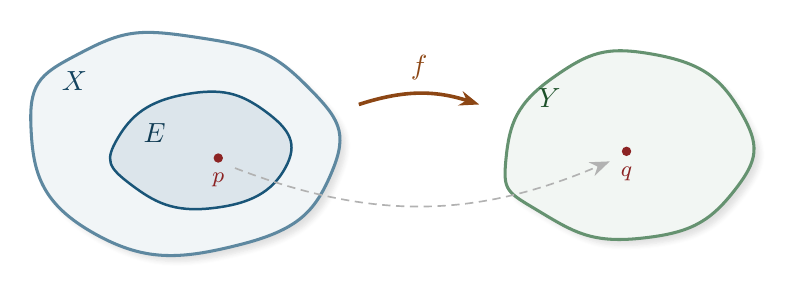
\begin{tikzpicture}[scale=0.85, >={Stealth[length=2.5mm]}]
    % --- Space X: organic blob, soft fill, subtle shadow ---
    \draw[defcolor!70, line width=1.1pt, fill=defcolor!6,
          blur shadow={shadow blur steps=6, shadow opacity=12}]
      plot [smooth cycle, tension=0.9] coordinates
      {(-2.2,0.3) (-1.4,1.4) (0.3,1.6) (1.9,0.9) (2.3,-0.4) (0.9,-1.5) (-1.3,-1.3)};
    \node[defcolor!80!black, font=\bfseries] at (-1.55,0.95) {$X$};
    % --- Subset E ---
    \draw[defcolor, line width=0.9pt, fill=defcolor!15]
      plot [smooth cycle, tension=0.9] coordinates
      {(-0.9,0.1) (0.1,0.75) (1.3,0.5) (1.6,-0.35) (0.5,-0.95) (-0.7,-0.6)};
    \node[defcolor!70!black] at (-0.35,0.18) {$E$};
    % --- p ---
    \fill[thmcolor] (0.6,-0.2) circle (2pt);
    \node[thmcolor, below=2pt] at (0.6,-0.2) {\footnotesize $p$};
    % --- mapping arrow ---
    \draw[->, mAccent, line width=1.3pt] (2.7,0.6) to[bend left=18]
      node[above=1pt, font=\itshape] {$f$} (4.5,0.6);
    % --- Space Y ---
    \draw[proofcolor!70, line width=1.1pt, fill=proofcolor!6,
          blur shadow={shadow blur steps=6, shadow opacity=12}]
      plot [smooth cycle, tension=0.9] coordinates
      {(4.9,-0.2) (5.6,1.0) (7.1,1.35) (8.4,0.5) (8.3,-0.7) (6.9,-1.4) (5.4,-1.0)};
    \node[proofcolor!80!black, font=\bfseries] at (5.55,0.7) {$Y$};
    % --- q ---
    \fill[thmcolor] (6.7,-0.1) circle (2pt);
    \node[thmcolor, below=2pt] at (6.7,-0.1) {\footnotesize $q$};
    % --- dashed trace: p is sent toward q ---
    \draw[->, gray!60, densely dashed, semithick]
      (0.85,-0.35) to[bend right=22] (6.45,-0.25);
  \end{tikzpicture}
  \end{center}

  \begin{hlbox}
  \textbf{Setting:} $f$ maps $E \subset X$ into $Y$, where $X$, $Y$ are \alert{metric spaces}.

  \vspace{0.3em}
  \textbf{Why so general?} Real, complex, and vector-valued functions are all
  special cases --- the general proofs are \emph{no harder}.
  \end{hlbox}

  \note{
    Here is the setting we will use throughout. In the picture, the blue
    region on the left is a metric space "X", and inside it sits a subset
    "E", shown in light blue. Our function "f" maps "E" into a second
    metric space "Y", the green region on the right. The point "p" lives
    in "X", and the candidate limit value "q" lives in "Y"; the dashed
    gray arrow suggests how "f" carries points near "p" toward "q". Why work at
    this level of generality? Because real functions, complex functions,
    and vector valued functions are all special cases, and the theorems
    would not become any easier if we restricted to real functions.
    Discarding unnecessary hypotheses actually clarifies the picture.
  }
\end{frame}
}

% =============================================================================
% THE DEFINITION
% =============================================================================
{
\usebackgroundtemplate{%
  
\includegraphics[width=\paperwidth,height=\paperheight,keepaspectratio=false]{chapter_04_bg_02.png}%
}
\section{The Definition of a Limit}

% --- Build 1/3 ---
\begin{frame}{Definition 4.1: Limit of a Function}
  \begin{defblock}{Definition 4.1}
    \small
    Let $X$ and $Y$ be metric spaces; suppose $E \subset X$, $f$ maps $E$ into $Y$,
    and $p$ is a \alert{limit point} of $E$.
  \end{defblock}

  \note{
    Here is the central definition of this section, built up in three
    steps. First, the cast of characters. "X" and "Y" are metric spaces,
    "E" is a subset of "X", and "f" maps "E" into "Y". Crucially, "p" must
    be a limit point of "E". This guarantees that there are points of "E"
    arbitrarily close to "p", so it makes sense to ask what happens as
    "x" approaches "p". Next, the notation.
  }
\end{frame}

% --- Build 2/3 ---
\begin{frame}{Definition 4.1: Limit of a Function}
  \begin{defblock}{Definition 4.1}
    \small
    Let $X$ and $Y$ be metric spaces; suppose $E \subset X$, $f$ maps $E$ into $Y$,
    and $p$ is a \alert{limit point} of $E$. We write $f(x) \to q$ as $x \to p$, or
    \begin{equation}
      \lim_{x \to p} f(x) = q \tag{1}
    \end{equation}
    if there is a point $q \in Y$ with the following property: \ldots
  \end{defblock}

  \note{
    We write "f" of "x" goes to "q" as "x" goes to "p", or, as equation 1
    shows, the limit of "f" of "x" as "x" approaches "p" equals "q". This
    holds when there is a point "q" in "Y" with a certain property, and
    that property is the famous epsilon delta condition, which we add now.
  }
\end{frame}

% --- Build 3/3 ---
\begin{frame}{Definition 4.1: Limit of a Function}
  \begin{defblock}{Definition 4.1}
    \small
    Let $X$ and $Y$ be metric spaces; suppose $E \subset X$, $f$ maps $E$ into $Y$,
    and $p$ is a \alert{limit point} of $E$. We write $f(x) \to q$ as $x \to p$, or
    \begin{equation}
      \lim_{x \to p} f(x) = q \tag{1}
    \end{equation}
    if there is a point $q \in Y$ with the following property:
    for every $\varepsilon > 0$ there exists a $\delta > 0$ such that
    \begin{equation}
      d_Y(f(x), q) < \varepsilon \tag{2}
    \end{equation}
    for all points $x \in E$ for which
    \begin{equation}
      0 < d_X(x, p) < \delta. \tag{3}
    \end{equation}
  \end{defblock}

  \note{
    Here is the full condition. For every positive epsilon there must
    exist a positive delta such that, as equation 2 says, the distance in
    "Y" between "f" of "x" and "q" is less than epsilon, for all points
    "x" in "E" satisfying equation 3, namely that the distance in "X"
    between "x" and "p" is strictly between zero and delta. Think of it
    as a challenge and response: no matter how small a target epsilon you
    demand around "q", I can find a radius delta around "p" so that "f"
    maps everything in that punctured ball into your target. Let us draw
    the picture.
  }
\end{frame}

\begin{frame}{The Picture in Metric Spaces}
  \begin{center}
  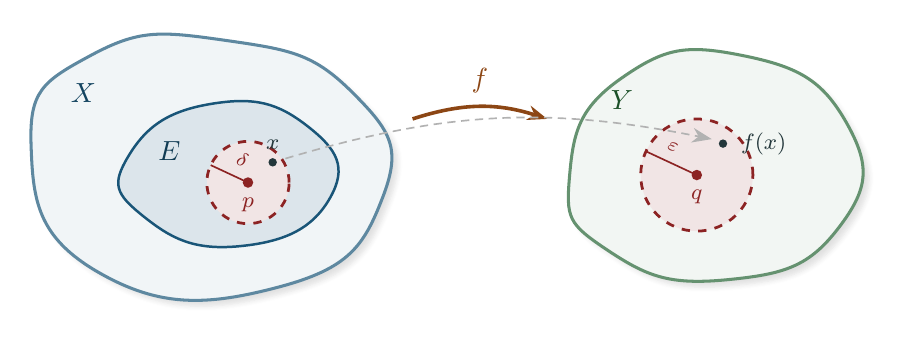
\begin{tikzpicture}[scale=0.95, >={Stealth[length=2.5mm]}]
    % --- Space X: organic blob ---
    \draw[defcolor!70, line width=1.1pt, fill=defcolor!6,
          blur shadow={shadow blur steps=6, shadow opacity=12}]
      plot [smooth cycle, tension=0.9] coordinates
      {(-2.3,0.3) (-1.5,1.5) (0.3,1.7) (2.0,1.0) (2.4,-0.4) (1.0,-1.6) (-1.4,-1.4)};
    \node[defcolor!80!black, font=\bfseries] at (-1.6,1.0) {$X$};
    \draw[defcolor, line width=0.9pt, fill=defcolor!15]
      plot [smooth cycle, tension=0.9] coordinates
      {(-1.0,0.15) (0.1,0.85) (1.4,0.55) (1.7,-0.4) (0.5,-1.05) (-0.8,-0.65)};
    \node[defcolor!70!black] at (-0.45,0.22) {$E$};
    % --- delta ball around p: soft halo + dashed rim + radius ---
    \fill[thmcolor!12] (0.6,-0.2) circle (0.55);
    \draw[thmcolor, dashed, line width=1pt] (0.6,-0.2) circle (0.55);
    \draw[thmcolor, semithick] (0.6,-0.2) --
      node[pos=0.35, above=0.5pt, sloped] {\scriptsize $\delta$} ++(155:0.55);
    \fill[thmcolor] (0.6,-0.2) circle (2pt);
    \node[thmcolor, below=2pt] at (0.6,-0.2) {\footnotesize $p$};
    % --- x ---
    \fill[mDarkTeal] (0.93,0.07) circle (1.6pt);
    \node[mDarkTeal, above=1pt] at (0.93,0.07) {\footnotesize $x$};
    % --- mapping arrow ---
    \draw[->, mAccent, line width=1.3pt] (2.8,0.65) to[bend left=18]
      node[above=1pt, font=\itshape] {$f$} (4.6,0.65);
    % --- Space Y: organic blob ---
    \draw[proofcolor!70, line width=1.1pt, fill=proofcolor!6,
          blur shadow={shadow blur steps=6, shadow opacity=12}]
      plot [smooth cycle, tension=0.9] coordinates
      {(4.9,-0.1) (5.6,1.2) (7.2,1.5) (8.6,0.6) (8.5,-0.8) (7.0,-1.5) (5.4,-1.1)};
    \node[proofcolor!80!black, font=\bfseries] at (5.6,0.9) {$Y$};
    % --- epsilon ball around q ---
    \fill[thmcolor!12] (6.6,-0.1) circle (0.75);
    \draw[thmcolor, dashed, line width=1pt] (6.6,-0.1) circle (0.75);
    \draw[thmcolor, semithick] (6.6,-0.1) --
      node[pos=0.6, above=0.5pt, sloped] {\scriptsize $\varepsilon$} ++(155:0.75);
    \fill[thmcolor] (6.6,-0.1) circle (2pt);
    \node[thmcolor, below=2pt] at (6.6,-0.1) {\footnotesize $q$};
    % --- f(x) ---
    \fill[mDarkTeal] (6.95,0.32) circle (1.6pt);
    \node[mDarkTeal, right=3pt] at (6.95,0.32) {\footnotesize $f(x)$};
    % --- dashed trace: x lands on f(x) ---
    \draw[->, gray!60, densely dashed, semithick]
      (1.1,0.12) to[bend left=14] (6.8,0.38);
  \end{tikzpicture}
  \end{center}

  \begin{hlbox}
  \textbf{Reading the definition:} every point $x \neq p$ inside the
  $\delta$-ball (and in $E$) is sent by $f$ into the $\varepsilon$-ball around $q$.
  \end{hlbox}

  \note{
    This diagram shows Definition 4.1 in action. On the left, the dashed
    red circle is the ball of radius delta around "p", drawn inside the
    metric space "X" with the set "E" in light blue; the short red
    segment marks its radius delta. On the right, the dashed red circle
    is the ball of radius epsilon around "q" in the space "Y". The
    definition demands that any point "x" of "E" lying inside the delta
    ball, other than "p" itself, gets mapped by "f" to a point "f" of "x"
    inside the epsilon ball; the gray dashed arrow traces one such point
    landing safely inside the target. The challenger picks epsilon on the
    right; we respond with delta on the left. Next, let us look at a
    concrete real function.
  }
\end{frame}

\begin{frame}{A Limit Where $f(p) \neq q$}
  \begin{center}
  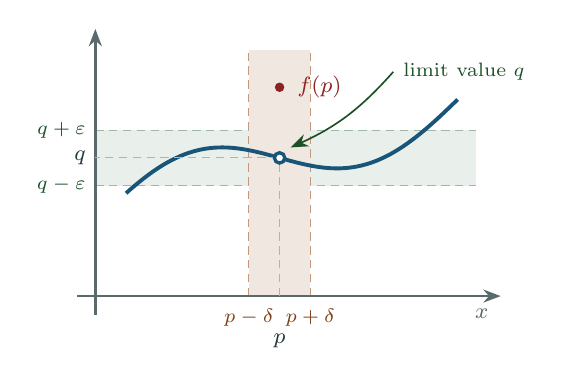
\begin{tikzpicture}[scale=0.78, >={Stealth[length=2.2mm]}]
    % --- bands first (epsilon: green, delta: warm orange) ---
    \fill[proofcolor!10] (0,1.8) rectangle (6.2,2.7);
    \draw[proofcolor!45, densely dashed, thin] (0,1.8) -- (6.2,1.8);
    \draw[proofcolor!45, densely dashed, thin] (0,2.7) -- (6.2,2.7);
    \fill[mAccent!13] (2.5,0) rectangle (3.5,4.0);
    \draw[mAccent!55, densely dashed, thin] (2.5,0) -- (2.5,4.0);
    \draw[mAccent!55, densely dashed, thin] (3.5,0) -- (3.5,4.0);
    % --- axes ---
    \draw[->, mDarkTeal!75, line width=0.9pt]
      (-0.3,0) -- (6.6,0) node[below left=1pt] {\footnotesize $x$};
    \draw[->, mDarkTeal!75, line width=0.9pt] (0,-0.3) -- (0,4.35);
    % --- curve ---
    \draw[defcolor, line width=1.4pt, domain=0.5:5.9, smooth, samples=80]
      plot (\x, {1.2 + 0.35*\x + 0.6*sin(\x*60)});
    % --- dashed guides to (p, q) ---
    \draw[gray!60, densely dashed] (3,0) -- (3,2.25) -- (0,2.25);
    % --- band labels ---
    \node[proofcolor!80!black, left] at (0,2.7) {\scriptsize $q + \varepsilon$};
    \node[proofcolor!80!black, left] at (0,1.8) {\scriptsize $q - \varepsilon$};
    \node[mDarkTeal, left] at (0,2.25) {\footnotesize $q$};
    \node[mAccent!90!black, below] at (2.5,-0.05) {\scriptsize $p - \delta$};
    \node[mAccent!90!black, below] at (3.5,-0.05) {\scriptsize $p + \delta$};
    \node[mDarkTeal, below] at (3,-0.45) {\footnotesize $p$};
    % --- annotation: the limit value (open circle) ---
    \draw[->, proofcolor!80!black, semithick]
      (4.85,3.65) node[right, font=\scriptsize, align=left] {limit value $q$}
      to[bend left=12] (3.18,2.42);
    % --- hole at (p, q): white-filled open circle on the curve ---
    \fill[white] (3,2.25) circle (2.4pt);
    \draw[defcolor, line width=1.2pt] (3,2.25) circle (2.4pt);
    % --- actual value f(p): deep red dot ---
    \fill[thmcolor] (3,3.4) circle (2.2pt);
    \node[thmcolor, right=3pt] at (3,3.4) {\footnotesize $f(p)$};
  \end{tikzpicture}
  \end{center}

  \begin{hlbox}
  $p$ need \alert{not} be in $E$; even if $p \in E$, possibly
  $f(p) \neq \lim\limits_{x \to p} f(x)$.
  \end{hlbox}

  \note{
    Here is the same idea for a real function. The blue curve is the
    graph of "f". The horizontal green band is the target zone between
    "q" minus epsilon and "q" plus epsilon, and the vertical orange band
    is the window between "p" minus delta and "p" plus delta. Inside the
    orange window, the curve stays within the green band, except possibly
    at "p" itself. Notice the open circle on the curve at "p", flagged by
    the small green arrow: the limit value "q" is where the curve is
    heading. But the red dot above shows
    the actual value "f" of "p", which is somewhere else entirely. The
    limit completely ignores what happens at "p"; that is why equation 3
    requires the distance to be strictly positive. Let us collect these
    observations as remarks.
  }
\end{frame}

% --- Build 1/3 ---
\begin{frame}{Remarks on Definition 4.1}
  \begin{remblock}{Remarks}
    \begin{itemize}
      \item $d_X$, $d_Y$ are the distances in $X$, $Y$.
        For $\mathbb{R}$, $\mathbb{C}$, $\mathbb{R}^k$: absolute values or norms
        of differences.
    \end{itemize}
  \end{remblock}

  \note{
    A few remarks about the definition. First, the symbols "d" sub "X"
    and "d" sub "Y" simply denote the distance functions of the two
    metric spaces. If "X" or "Y" happens to be the real line, the complex
    plane, or a euclidean space, the distances are replaced by absolute
    values or by norms of differences, exactly as in Chapter 2.
  }
\end{frame}

% --- Build 2/3 ---
\begin{frame}{Remarks on Definition 4.1}
  \begin{remblock}{Remarks}
    \begin{itemize}
      \item $d_X$, $d_Y$ are the distances in $X$, $Y$.
        For $\mathbb{R}$, $\mathbb{C}$, $\mathbb{R}^k$: absolute values or norms
        of differences.
      \item $p \in X$ must be a limit point of $E$, but $p$ \alert{need not
        belong to $E$}.
    \end{itemize}
  \end{remblock}

  \note{
    Second, observe that "p" is required to be a point of "X" and a limit
    point of "E", but it does not have to belong to "E" at all. The
    function may be entirely undefined at "p", and the limit can still
    exist. For example, the function sine of "x", divided by "x", is
    undefined at zero, yet its limit at zero exists and equals 1.
  }
\end{frame}

% --- Build 3/3 ---
\begin{frame}{Remarks on Definition 4.1}
  \begin{remblock}{Remarks}
    \begin{itemize}
      \item $d_X$, $d_Y$ are the distances in $X$, $Y$.
        For $\mathbb{R}$, $\mathbb{C}$, $\mathbb{R}^k$: absolute values or norms
        of differences.
      \item $p \in X$ must be a limit point of $E$, but $p$ \alert{need not
        belong to $E$}.
      \item Even if $p \in E$, possibly $f(p) \neq \lim\limits_{x \to p} f(x)$:
        condition (3) \alert{excludes $x = p$}.
    \end{itemize}
  \end{remblock}

  \note{
    Third, even when "p" does belong to "E", the value "f" of "p" plays
    no role whatsoever in the definition. The strict inequality in
    equation 3, that the distance is greater than zero, excludes the
    point "x" equals "p" from consideration. So the limit may exist and
    differ from "f" of "p". As we will see in the next section, when the
    two do agree we call the function continuous at "p". Now let us
    connect function limits to sequence limits.
  }
\end{frame}
}

% =============================================================================
% LIMITS VIA SEQUENCES
% =============================================================================
{
\usebackgroundtemplate{%
  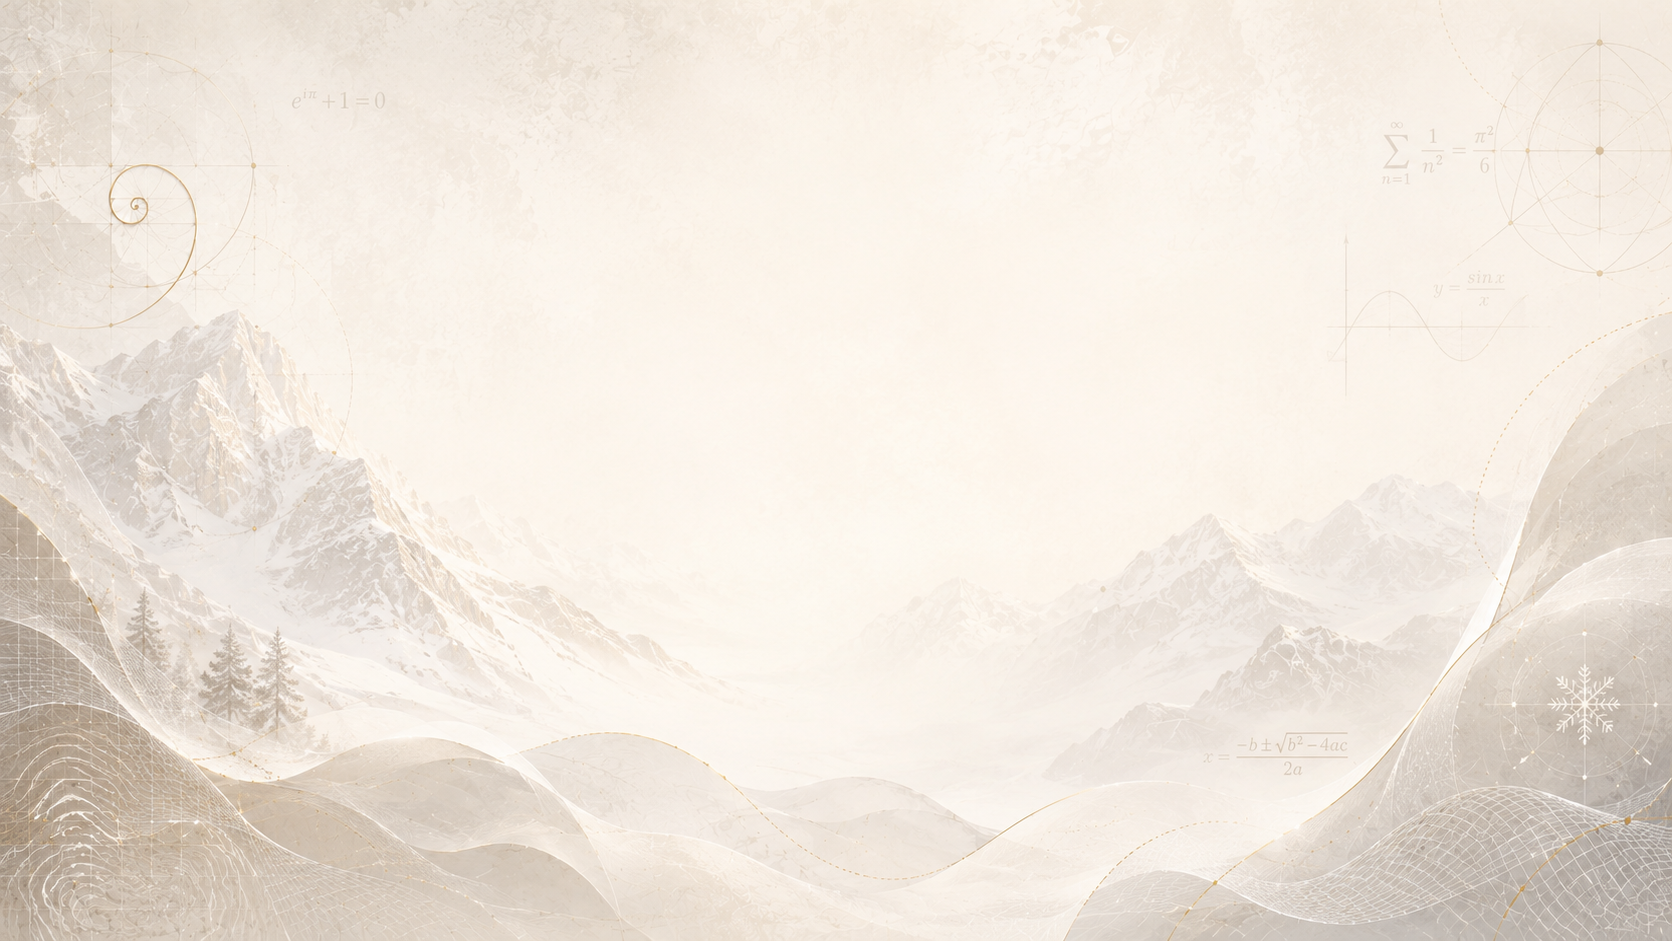
\includegraphics[width=\paperwidth,height=\paperheight,keepaspectratio=false]{chapter_04_bg_03.png}%
}
\section{Limits via Sequences}

\begin{frame}{Theorem 4.2: Sequential Characterization}
  \begin{thmblock}{Theorem 4.2}
    Let $X$, $Y$, $E$, $f$, and $p$ be as in Definition 4.1. Then
    \begin{equation}
      \lim_{x \to p} f(x) = q \tag{4}
    \end{equation}
    if and only if
    \begin{equation}
      \lim_{n \to \infty} f(p_n) = q \tag{5}
    \end{equation}
    for \alert{every} sequence $\{p_n\}$ in $E$ such that
    \begin{equation}
      p_n \neq p, \qquad \lim_{n \to \infty} p_n = p. \tag{6}
    \end{equation}
  \end{thmblock}

  \note{
    Here is the main theorem of this section. It says that the epsilon
    delta statement, equation 4, holds if and only if equation 5 holds:
    the image sequence "f" of "p" sub "n" converges to "q" for every
    sequence "p" sub "n" in "E" that satisfies equation 6, meaning the
    terms avoid "p" but converge to "p". The word every is essential; a
    single well-behaved sequence proves nothing. The power of this
    theorem is that it converts statements about function limits into
    statements about sequence limits, where we already have a full
    toolbox from Chapter 3. Let us see the proof strategy.
  }
\end{frame}

\begin{frame}{Proof Strategy: Theorem 4.2}
  \begin{hlbox}
  \textbf{Goal:} Prove the equivalence (4) $\iff$ (5).

  \vspace{0.8em}
  \begin{enumerate}
    \item \textbf{($\Rightarrow$)} Assume (4). Chain the two definitions:
      $\varepsilon \rightsquigarrow \delta \rightsquigarrow N$.
    \item \textbf{($\Leftarrow$)} Prove the contrapositive: if (4) \alert{fails},
      build a \alert{bad sequence} with $\delta_n = 1/n$.
  \end{enumerate}

  \vspace{0.8em}
  \textbf{Technique:} the second half is a classic
  \alert{sequence-construction}.
  \end{hlbox}

  \note{
    The proof has two halves. The forward direction is a routine chaining
    of definitions: given epsilon, the function limit hands us a delta,
    and the sequence convergence hands us an index "N" beyond which the
    terms are within delta of "p". The converse is proved in
    contrapositive form: assuming the function limit fails, we must
    manufacture a single sequence that converges to "p" while its image
    refuses to converge to "q". The trick is to shrink delta along the
    values 1 over "n" and harvest one bad point at each stage. Let us
    carry out the forward direction first.
  }
\end{frame}

% --- Build 1/2 ---
\begin{frame}{Proof of Theorem 4.2 --- ($\Rightarrow$)}
  \begin{proofblock}{Step 1: From $\varepsilon$ to $\delta$}
    Suppose (4) holds. Choose $\{p_n\}$ in $E$ satisfying (6).
    Let $\varepsilon > 0$ be given. Then there exists $\delta > 0$ such that
    \[
      d_Y(f(x), q) < \varepsilon \quad \text{if } x \in E \text{ and }
      0 < d_X(x, p) < \delta.
    \]
  \end{proofblock}

  \note{
    Assume the function limit, equation 4, holds, and fix any sequence
    "p" sub "n" in "E" satisfying equation 6. Let a positive epsilon be
    given. By Definition 4.1 there is a positive delta such that "f"
    carries every point of "E" within distance delta of "p", excluding
    "p" itself, to within epsilon of "q". Next we bring the sequence
    into play.
  }
\end{frame}

% --- Build 2/2 ---
\begin{frame}{Proof of Theorem 4.2 --- ($\Rightarrow$)}
  \begin{proofblock}{Step 1: From $\varepsilon$ to $\delta$}
    Suppose (4) holds. Choose $\{p_n\}$ in $E$ satisfying (6).
    Let $\varepsilon > 0$ be given. Then there exists $\delta > 0$ such that
    \[
      d_Y(f(x), q) < \varepsilon \quad \text{if } x \in E \text{ and }
      0 < d_X(x, p) < \delta.
    \]
  \end{proofblock}

  \begin{proofblock}{Step 2: From $\delta$ to $N$}
    Since $p_n \to p$ and $p_n \neq p$, there exists $N$ such that
    \[
      n > N \;\Longrightarrow\; 0 < d_X(p_n, p) < \delta
      \;\Longrightarrow\; d_Y(f(p_n), q) < \varepsilon.
    \]
    Hence $f(p_n) \to q$, i.e., (5) holds. \hfill $\blacksquare$~(forward direction)
  \end{proofblock}

  \note{
    Now use the convergence of the sequence: there exists an index "N"
    such that for all "n" greater than "N", the distance from "p" sub "n"
    to "p" is less than delta, and it is positive because the terms never
    equal "p". So each such "p" sub "n" qualifies for the delta condition
    from step 1, which forces "f" of "p" sub "n" to lie within epsilon of
    "q". Since epsilon was arbitrary, the image sequence converges to
    "q", which is exactly equation 5. The forward direction is done. Now
    for the converse.
  }
\end{frame}

% --- Build 1/2 ---
\begin{frame}{Proof of Theorem 4.2 --- ($\Leftarrow$), by Contraposition}
  \begin{proofblock}{Step 1: Negate (4)}
    Suppose (4) is \alert{false}. Then there exists some $\varepsilon > 0$ such
    that for \alert{every} $\delta > 0$ there is a point $x \in E$
    (depending on $\delta$) with
    \[
      d_Y(f(x), q) \geq \varepsilon
      \quad \text{but} \quad 0 < d_X(x, p) < \delta.
    \]
  \end{proofblock}

  \note{
    For the converse we argue by contraposition: assuming equation 4
    fails, we will show equation 5 fails for some sequence. Negating the
    definition carefully: there is one stubborn epsilon such that no
    delta works. That is, for every positive delta, some point "x" of
    "E" lies within delta of "p", without being "p", and yet its image
    stays at distance at least epsilon from "q". Now we turn this failure
    into a sequence.
  }
\end{frame}

% --- Build 2/2 ---
\begin{frame}{Proof of Theorem 4.2 --- ($\Leftarrow$), by Contraposition}
  \begin{proofblock}{Step 1: Negate (4)}
    Suppose (4) is \alert{false}. Then there exists some $\varepsilon > 0$ such
    that for \alert{every} $\delta > 0$ there is a point $x \in E$
    (depending on $\delta$) with
    \[
      d_Y(f(x), q) \geq \varepsilon
      \quad \text{but} \quad 0 < d_X(x, p) < \delta.
    \]
  \end{proofblock}

  \begin{proofblock}{Step 2: Build the bad sequence}
    Take $\delta_n = \tfrac{1}{n}$ $(n = 1, 2, 3, \dots)$: we obtain points
    $p_n \in E$ with $0 < d_X(p_n, p) < \tfrac{1}{n}$ but
    $d_Y(f(p_n), q) \geq \varepsilon$.

    \smallskip
    The sequence $\{p_n\}$ satisfies (6), yet (5) is \alert{false}.
    \hfill $\blacksquare$
  \end{proofblock}

  \note{
    Apply the failure with delta equal to 1 over "n", for each positive
    integer "n". At every stage we harvest a point "p" sub "n" of "E"
    that is within 1 over "n" of "p", but not equal to "p", whose image
    remains at distance at least epsilon from "q". The resulting sequence
    converges to "p" and avoids "p", so it satisfies equation 6, yet its
    image sequence stays away from "q" forever, so equation 5 fails.
    That completes the contrapositive, and with it the whole theorem.
    An important corollary drops out immediately.
  }
\end{frame}

\begin{frame}{Corollary: Uniqueness of Limits}
  \begin{thmblock}{Corollary}
    If $f$ has a limit at $p$, this limit is \alert{unique}.
  \end{thmblock}

  \vspace{0.6em}
  \hl{\textbf{Why:} Theorem 3.2($b$) (limits of sequences are unique)
  $+$ Theorem 4.2.}

  \vspace{0.6em}
  \begin{remblock}{Recall: Theorem 3.2(b)}
    A sequence in a metric space converges to \emph{at most one} point.
  \end{remblock}

  \note{
    The corollary states that a function can have at most one limit at a
    given point. The proof, shown on the slide, takes a single line. Since "p"
    is a limit point of "E", there exists at least one sequence in "E"
    converging to "p" without hitting it. By Theorem 4.2, any limit of
    "f" at "p" must also be the limit of the image sequence. But the
    recall box reminds us of Theorem 3.2 part "b": a sequence in a metric
    space converges to at most one point. So two different function
    limits would force one sequence to have two different limits, which
    is impossible. Next, let us watch the sequential criterion in action
    on a famous example.
  }
\end{frame}

% --- Build 1/3 ---
\begin{frame}{Example: A Limit That Fails to Exist}
  \begin{exblock}{Example (the criterion in action)}
    \small
    Does $\displaystyle\lim_{x \to 0} \sin\!\Big(\frac{1}{x}\Big)$ exist?
    \quad Here $E = (0, 1]$; note $0 \notin E$, but $0$ \emph{is} a limit point of $E$.
  \end{exblock}

  \begin{center}
  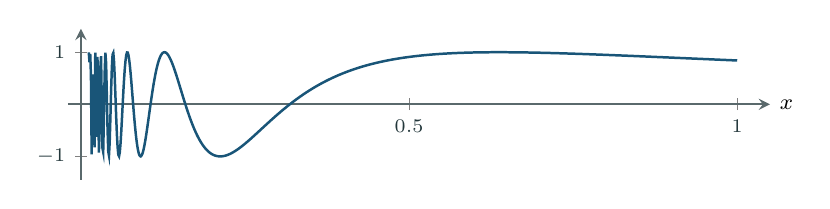
\begin{tikzpicture}
    \begin{axis}[
      width=10.5cm, height=3.5cm,
      axis lines=middle,
      xmin=-0.02, xmax=1.05, ymin=-1.45, ymax=1.45,
      xtick={0.5,1}, ytick={-1,1},
      tick label style={font=\scriptsize, color=mDarkTeal},
      axis line style={mDarkTeal!75, line width=0.8pt},
      xlabel={\footnotesize $x$}, x label style={anchor=west},
    ]
      \addplot[defcolor, line width=0.9pt, domain=0.012:1, samples=900]
        {sin(deg(1/x))};
    \end{axis}
  \end{tikzpicture}
  \end{center}

  \note{
    Let us see the sequential criterion earn its keep on a famous
    example. Consider sine of the quantity 1 over "x", defined on the
    half open interval from 0 to 1. The point zero is not in the domain, but it is
    a limit point of the domain, so the question on the slide makes
    sense: does the limit at zero exist? The graph tells the story. As
    "x" shrinks toward zero, 1 over "x" blows up, so the function
    oscillates between minus 1 and plus 1 faster and faster. Let us
    probe this oscillation with sequences.
  }
\end{frame}

% --- Build 2/3 ---
\begin{frame}{Example: A Limit That Fails to Exist}
  \begin{exblock}{Example (the criterion in action)}
    \small
    Does $\displaystyle\lim_{x \to 0} \sin\!\Big(\frac{1}{x}\Big)$ exist?
    \quad Here $E = (0, 1]$; note $0 \notin E$, but $0$ \emph{is} a limit point of $E$.
  \end{exblock}

  \begin{center}
  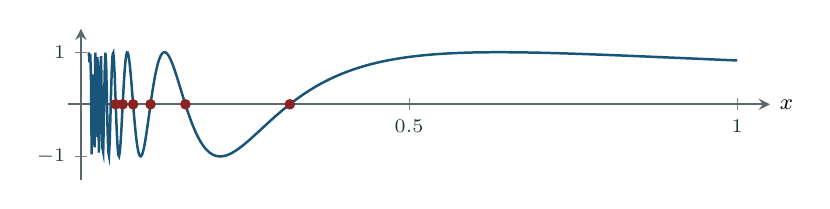
\begin{tikzpicture}
    \begin{axis}[
      width=10.5cm, height=3.5cm,
      axis lines=middle,
      xmin=-0.02, xmax=1.05, ymin=-1.45, ymax=1.45,
      xtick={0.5,1}, ytick={-1,1},
      tick label style={font=\scriptsize, color=mDarkTeal},
      axis line style={mDarkTeal!75, line width=0.8pt},
      xlabel={\footnotesize $x$}, x label style={anchor=west},
    ]
      \addplot[defcolor, line width=0.9pt, domain=0.012:1, samples=900]
        {sin(deg(1/x))};
      \addplot[only marks, mark=*, mark size=1.7pt, thmcolor] coordinates
        {(0.3183,0) (0.1592,0) (0.1061,0) (0.0796,0) (0.0637,0) (0.0531,0)};
    \end{axis}
  \end{tikzpicture}
  \end{center}

  \vspace{-0.4em}
  \begin{hlbox}
  {\small
  \textcolor{thmcolor}{$\bullet$} Along
  $a_n = \frac{1}{n\pi} \to 0$:\; $f(a_n) = \sin(n\pi) = 0 \;\to\; 0$
  }
  \end{hlbox}

  \note{
    First probe: the red dots on the graph. Take "a" sub "n" equal to 1
    over "n" pi. This sequence lives in the domain, never equals zero,
    and converges to zero, so it satisfies condition 6. At each of these
    points, sine of "n" pi is exactly zero, so the image sequence is
    constantly zero and converges to zero. If we looked only at this
    sequence, we might guess the limit is zero. But the theorem demands
    that every sequence agree. Let us try a second one.
  }
\end{frame}

% --- Build 3/3 ---
\begin{frame}{Example: A Limit That Fails to Exist}
  \begin{exblock}{Example (the criterion in action)}
    \small
    Does $\displaystyle\lim_{x \to 0} \sin\!\Big(\frac{1}{x}\Big)$ exist?
    \quad Here $E = (0, 1]$; note $0 \notin E$, but $0$ \emph{is} a limit point of $E$.
  \end{exblock}

  \begin{center}
  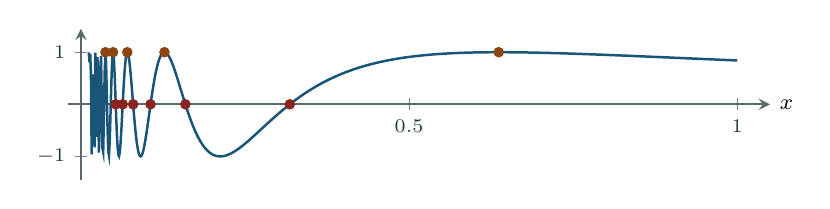
\begin{tikzpicture}
    \begin{axis}[
      width=10.5cm, height=3.5cm,
      axis lines=middle,
      xmin=-0.02, xmax=1.05, ymin=-1.45, ymax=1.45,
      xtick={0.5,1}, ytick={-1,1},
      tick label style={font=\scriptsize, color=mDarkTeal},
      axis line style={mDarkTeal!75, line width=0.8pt},
      xlabel={\footnotesize $x$}, x label style={anchor=west},
    ]
      \addplot[defcolor, line width=0.9pt, domain=0.012:1, samples=900]
        {sin(deg(1/x))};
      \addplot[only marks, mark=*, mark size=1.7pt, thmcolor] coordinates
        {(0.3183,0) (0.1592,0) (0.1061,0) (0.0796,0) (0.0637,0) (0.0531,0)};
      \addplot[only marks, mark=*, mark size=1.7pt, mAccent] coordinates
        {(0.6366,1) (0.1273,1) (0.0707,1) (0.0490,1) (0.0374,1)};
    \end{axis}
  \end{tikzpicture}
  \end{center}

  \vspace{-0.4em}
  \begin{hlbox}
  {\small
  \textcolor{thmcolor}{$\bullet$} Along
  $a_n = \frac{1}{n\pi} \to 0$:\; $f(a_n) = \sin(n\pi) = 0 \;\to\; 0$\\
  \textcolor{mAccent}{$\bullet$} Along
  $b_n = \frac{2}{(4n+1)\pi} \to 0$:\;
  $f(b_n) = \sin\big(2n\pi + \tfrac{\pi}{2}\big) = 1 \;\to\; 1$

  \smallskip
  Two sequences, two different limits $\;\Longrightarrow\;$ \\
  by Theorem 4.2, the limit does \alert{not exist}.
  }
  \end{hlbox}

  \note{
    Second probe: the orange dots. Take "b" sub "n" equal to 2 over the
    quantity 4 "n" plus 1, times pi. This sequence also converges to
    zero inside the domain, but now sine evaluates to exactly 1 at every
    term, so the image sequence converges to 1. Two perfectly legitimate
    sequences produce two different limits, zero and 1. By Theorem 4.2,
    the limit of sine of the quantity 1 over "x" at zero does not exist. With the
    structural theory in place, we now turn to the arithmetic of limits.
  }
\end{frame}
}

% =============================================================================
% ALGEBRA OF FUNCTIONS
% =============================================================================
{
\usebackgroundtemplate{%
  
\includegraphics[width=\paperwidth,height=\paperheight,keepaspectratio=false]{chapter_04_bg_04.png}%
}
\section{The Algebra of Functions}

% --- Build 1/2 ---
\begin{frame}{Definition 4.3: Operations on Functions}
  \begin{defblock}{Definition 4.3 (complex functions)}
    Let $f, g \colon E \to \mathbb{C}$. Define, for each $x \in E$:
    \[
      (f+g)(x) = f(x) + g(x), \qquad (f-g)(x) = f(x) - g(x),
    \]
    \[
      (fg)(x) = f(x)\,g(x), \qquad
      \left(\frac{f}{g}\right)(x) = \frac{f(x)}{g(x)}
      \;\; \text{(only where } g(x) \neq 0\text{)}.
    \]
  \end{defblock}

  \note{
    Before stating the limit laws we need to say precisely what it means
    to add or multiply two functions. Given two complex functions "f" and
    "g" defined on the same set "E", their sum assigns to each point "x"
    the number "f" of "x" plus "g" of "x", and similarly for the
    difference and the product. The quotient "f" over "g" is defined only
    at those points "x" of "E" where "g" of "x" is not zero. Everything
    is done pointwise. Two more pieces of notation complete the picture.
  }
\end{frame}

% --- Build 2/2 ---
\begin{frame}{Definition 4.3: Operations on Functions}
  \begin{defblock}{Definition 4.3 (complex functions)}
    Let $f, g \colon E \to \mathbb{C}$. Define, for each $x \in E$:
    \[
      (f+g)(x) = f(x) + g(x), \qquad (f-g)(x) = f(x) - g(x),
    \]
    \[
      (fg)(x) = f(x)\,g(x), \qquad
      \left(\frac{f}{g}\right)(x) = \frac{f(x)}{g(x)}
      \;\; \text{(only where } g(x) \neq 0\text{)}.
    \]
  \end{defblock}

  \begin{defblock}{Notation}
    \begin{itemize}
      \item $f = c$: \emph{constant} function, $f(x) = c$ for all $x \in E$.
      \item $f \geq g$ (real $f$, $g$): means $f(x) \geq g(x)$ for every $x \in E$.
    \end{itemize}
  \end{defblock}

  \note{
    Two abbreviations. If "f" assigns the same number "c" to every point
    of "E", we call "f" a constant function and simply write "f" equals
    "c". And if "f" and "g" are real functions with "f" of "x" greater
    than or equal to "g" of "x" at every point of "E", we write "f" is
    greater than or equal to "g" for brevity. There are analogous
    operations for vector valued functions, which we record next.
  }
\end{frame}

\begin{frame}{Definition 4.3: Vector-Valued Functions}
  \begin{defblock}{Definition 4.3 (vector-valued functions)}
    If $\mathbf{f}, \mathbf{g} \colon E \to \mathbb{R}^k$, define
    \[
      (\mathbf{f} + \mathbf{g})(x) = \mathbf{f}(x) + \mathbf{g}(x), \qquad
      (\mathbf{f} \cdot \mathbf{g})(x) = \mathbf{f}(x) \cdot \mathbf{g}(x),
    \]
    and for $\lambda \in \mathbb{R}$,
    $\;(\lambda \mathbf{f})(x) = \lambda\, \mathbf{f}(x)$.
  \end{defblock}

  \vspace{0.5em}
  \hl{Note: $\mathbf{f} \cdot \mathbf{g}$ is the \alert{inner product} --- a
  \emph{scalar}-valued function.}

  \note{
    For functions taking values in "k" dimensional euclidean space, the
    sum is again defined pointwise, and the dot product of "f" and "g"
    assigns to "x" the inner product of the two vectors "f" of "x" and
    "g" of "x". Notice that this dot product is a scalar valued function,
    not a vector valued one. Finally, multiplying by a real number lambda
    simply scales the function pointwise. With the algebra in place, here
    come the limit laws.
  }
\end{frame}

% --- Build 1/3 ---
\begin{frame}{Theorem 4.4: Limit Laws}
  \begin{thmblock}{Theorem 4.4}
    \small
    Suppose $E \subset X$, a metric space, $p$ is a limit point of $E$,
    $f$ and $g$ are complex functions on $E$, and
    \[
      \lim_{x \to p} f(x) = A, \qquad \lim_{x \to p} g(x) = B.
    \]
    Then:
    \begin{enumerate}
      \item[(a)] $\displaystyle\lim_{x \to p} (f + g)(x) = A + B$;
    \end{enumerate}
  \end{thmblock}

  \note{
    Theorem 4.4 is the workhorse for computing limits. The hypotheses:
    "E" is a subset of a metric space, "p" is a limit point of "E", and
    "f" and "g" are complex functions on "E" whose limits at "p" exist
    and equal "A" and "B" respectively. The first conclusion, part "a",
    says the limit of the sum is the sum of the limits, "A" plus "B".
    Two more laws follow.
  }
\end{frame}

% --- Build 2/3 ---
\begin{frame}{Theorem 4.4: Limit Laws}
  \begin{thmblock}{Theorem 4.4}
    \small
    Suppose $E \subset X$, a metric space, $p$ is a limit point of $E$,
    $f$ and $g$ are complex functions on $E$, and
    \[
      \lim_{x \to p} f(x) = A, \qquad \lim_{x \to p} g(x) = B.
    \]
    Then:
    \begin{enumerate}
      \item[(a)] $\displaystyle\lim_{x \to p} (f + g)(x) = A + B$;
      \item[(b)] $\displaystyle\lim_{x \to p} (fg)(x) = AB$;
    \end{enumerate}
  \end{thmblock}

  \note{
    Part "b" says the limit of the product is the product of the limits,
    "A" times "B". Notice there is no assumption that the limits are
    nonzero or that the functions are bounded; existence of the two
    limits is all we need. One more law, for quotients.
  }
\end{frame}

% --- Build 3/3 ---
\begin{frame}{Theorem 4.4: Limit Laws}
  \begin{thmblock}{Theorem 4.4}
    \small
    Suppose $E \subset X$, a metric space, $p$ is a limit point of $E$,
    $f$ and $g$ are complex functions on $E$, and
    \[
      \lim_{x \to p} f(x) = A, \qquad \lim_{x \to p} g(x) = B.
    \]
    Then:
    \begin{enumerate}
      \item[(a)] $\displaystyle\lim_{x \to p} (f + g)(x) = A + B$;
      \item[(b)] $\displaystyle\lim_{x \to p} (fg)(x) = AB$;
      \item[(c)] $\displaystyle\lim_{x \to p} \left(\frac{f}{g}\right)(x)
        = \frac{A}{B}$, \; if $B \neq 0$.
    \end{enumerate}
  \end{thmblock}

  \note{
    Part "c" handles quotients: the limit of "f" over "g" is "A" over
    "B", provided "B" is not zero. The restriction is clearly necessary,
    since we cannot divide by zero in the target. Together these three
    laws let us compute limits of any rational combination of functions
    from the limits of the pieces. And thanks to Theorem 4.2, the proof
    costs us almost nothing.
  }
\end{frame}

\begin{frame}{Proof of Theorem 4.4}
  \begin{proofblock}{Proof}
    In view of Theorem 4.2, these assertions follow immediately from the
    analogous properties of \alert{sequences} (Theorem 3.3).
    \hfill $\blacksquare$
  \end{proofblock}

  \vspace{0.6em}
  \begin{hlbox}
  \textbf{The bridge in action:}
  \[
    \text{(4) function limit}
    \;\overset{\text{Thm 4.2}}{\longleftrightarrow}\;
    \text{(5) sequence limits}
    \;\overset{\text{Thm 3.3}}{\longleftrightarrow}\;
    \text{limit laws}
  \]
  \end{hlbox}

  \note{
    Here is the payoff of the sequential characterization. To prove part
    "a", take any sequence "p" sub "n" converging to "p" in "E" without
    hitting "p". By Theorem 4.2, "f" of "p" sub "n" tends to "A" and "g"
    of "p" sub "n" tends to "B". Theorem 3.3 from Chapter 3 tells us that
    sums, products, and quotients of convergent sequences behave exactly
    as expected, so the image sequence of "f" plus "g" tends to "A" plus
    "B". Since the sequence was arbitrary, Theorem 4.2 converts this back
    into the function limit statement. The same argument proves parts
    "b" and "c". No new epsilon delta work is needed; that is the bridge
    in action, as the diagram on the slide shows.
  }
\end{frame}

\begin{frame}{Remark: Vector-Valued Limit Laws}
  \begin{remblock}{Remark}
    If $\mathbf{f}$ and $\mathbf{g}$ map $E$ into $\mathbb{R}^k$, then
    ($a$) remains true, and ($b$) becomes:
    \begin{enumerate}
      \item[($b'$)] $\displaystyle\lim_{x \to p}
        (\mathbf{f} \cdot \mathbf{g})(x) = \mathbf{A} \cdot \mathbf{B}$.
    \end{enumerate}
    (Compare Theorem 3.4.) There is no analogue of ($c$): we cannot
    divide by a vector.
  \end{remblock}

  \note{
    A closing remark on the vector valued case. If "f" and "g" take
    values in "k" dimensional euclidean space, the sum law, part "a",
    remains true word for word, and the product law becomes part "b"
    prime: the limit of the dot product is the dot product of the limit
    vectors. This parallels Theorem 3.4 about sequences in euclidean
    spaces. There is no quotient law, of course, since division by a
    vector is undefined. That completes the mathematical content of this
    section; let us summarize.
  }
\end{frame}
}

% =============================================================================
% SUMMARY
% =============================================================================
{
\usebackgroundtemplate{%
  
\includegraphics[width=\paperwidth,height=\paperheight,keepaspectratio=false]{chapter_04_bg_05.png}%
}
\section{Summary}

% --- Build 1/3 ---
\begin{frame}{Summary}
  \begin{hlbox}
  \textbf{Key takeaways from this section:}
  \begin{itemize}
    \item \alert{Definition 4.1}: $\lim_{x \to p} f(x) = q$ via
      $\varepsilon$--$\delta$ in metric spaces; $p$ a limit point of $E$,
      value $f(p)$ \emph{irrelevant}
  \end{itemize}
  \end{hlbox}

  \note{
    Let us review what we covered. First, Definition 4.1 gave the epsilon
    delta definition of a function limit between metric spaces. The point
    "p" must be a limit point of the domain "E", but it need not belong
    to "E", and even when it does, the value of "f" at "p" plays no role
    in the limit.
  }
\end{frame}

% --- Build 2/3 ---
\begin{frame}{Summary}
  \begin{hlbox}
  \textbf{Key takeaways from this section:}
  \begin{itemize}
    \item \alert{Definition 4.1}: $\lim_{x \to p} f(x) = q$ via
      $\varepsilon$--$\delta$ in metric spaces; $p$ a limit point of $E$,
      value $f(p)$ \emph{irrelevant}
    \item \alert{Theorem 4.2}: function limits $\iff$ sequence limits;
      corollary: limits are \emph{unique}
  \end{itemize}
  \end{hlbox}

  \note{
    Second, Theorem 4.2 showed that the function limit equals "q" exactly
    when every sequence approaching "p" inside "E", while avoiding "p",
    has its image converge to "q". This bridge to Chapter 3 immediately
    gave us the corollary that limits, when they exist, are unique.
  }
\end{frame}

% --- Build 3/3 ---
\begin{frame}{Summary}
  \begin{hlbox}
  \textbf{Key takeaways from this section:}
  \begin{itemize}
    \item \alert{Definition 4.1}: $\lim_{x \to p} f(x) = q$ via
      $\varepsilon$--$\delta$ in metric spaces; $p$ a limit point of $E$,
      value $f(p)$ \emph{irrelevant}
    \item \alert{Theorem 4.2}: function limits $\iff$ sequence limits;
      corollary: limits are \emph{unique}
    \item \alert{Theorem 4.4}: limit laws for $f + g$, $fg$, $f/g$
      (and $\mathbf{f} + \mathbf{g}$, $\mathbf{f} \cdot \mathbf{g}$)
  \end{itemize}

  \vspace{0.8em}
  \textbf{Coming up next:}\\
  \emph{Continuous Functions} --- what happens when
  $\lim_{x \to p} f(x) = f(p)$.
  \end{hlbox}

  \note{
    Third, Theorem 4.4 established the limit laws: limits respect sums,
    products, and quotients of complex functions, with the analogous sum
    and dot product laws for vector valued functions. The proofs were
    nearly free, courtesy of the sequential characterization. In the next
    section we take the decisive step: a function is continuous at "p"
    precisely when its limit at "p" exists and equals its value there.
    See you in the next episode.
  }
\end{frame}
}

\end{document}
